\documentclass[final]{article}

\usepackage[paperwidth=60in,paperheight=36in,margin=0.5in]{geometry}
\usepackage{fix-cm}
\usepackage[T1]{fontenc}
\usepackage[default,scaled=0.92]{sourcecodepro}
\usepackage{amsmath,amssymb}
\usepackage{graphicx}
\usepackage{xcolor}
\usepackage{tikz}
\usepackage{array,booktabs}
\usepackage{enumitem}
\usepackage[most]{tcolorbox}
\usetikzlibrary{calc}

\pagestyle{empty}
\setlength{\parindent}{0pt}
\setlength{\parskip}{0.18em}
\setlength{\abovedisplayskip}{0.10in}
\setlength{\belowdisplayskip}{0.10in}
\setlength{\abovedisplayshortskip}{0.07in}
\setlength{\belowdisplayshortskip}{0.07in}

\definecolor{posterbg}{HTML}{FFFFFF}
\definecolor{ink}{HTML}{000000}
\definecolor{muted}{HTML}{5F5F5F}
\definecolor{teal}{HTML}{000000}
\definecolor{teallight}{HTML}{F2F2F2}
\definecolor{amber}{HTML}{202020}
\definecolor{amberlight}{HTML}{F7F7F7}
\definecolor{red}{HTML}{303030}
\definecolor{redlight}{HTML}{F4F4F4}
\definecolor{blue}{HTML}{111111}
\definecolor{bluelight}{HTML}{ECECEC}
\definecolor{border}{HTML}{000000}

\pagecolor{posterbg}
\color{ink}

\newcommand{\TitleFont}{\fontsize{52}{60}\selectfont}
\newcommand{\AuthorFont}{\fontsize{27}{32}\selectfont}
\newcommand{\BodyFont}{\fontsize{34}{40}\selectfont}
\newcommand{\SmallFont}{\fontsize{28}{33}\selectfont}
\newcommand{\TinyFont}{\fontsize{24}{29}\selectfont}
\newcommand{\ClaimFont}{\fontsize{32}{37}\selectfont}
\newcommand{\SectionFont}{\fontsize{46}{52}\selectfont\bfseries}
\newcommand{\SubheadFont}{\fontsize{36}{42}\selectfont\bfseries}
\newcommand{\MiniHeadFont}{\fontsize{32}{37}\selectfont\bfseries}
\newcommand{\EquationFont}{\fontsize{36}{42}\selectfont}
\newcommand{\TableFont}{\fontsize{25}{30}\selectfont}

\tcbset{
  colback=white,
  colframe=border,
  boxrule=1.15pt,
  arc=0mm,
  outer arc=0mm,
  sharp corners,
  left=7mm,
  right=7mm,
  top=5mm,
  bottom=5mm,
  boxsep=0mm,
  defblock/.style={colback=bluelight, colframe=border},
  resultblock/.style={colback=white, colframe=border},
  witnessblock/.style={colback=teallight, colframe=teallight, boxrule=0pt},
  takeawayblock/.style={colback=black, colframe=black, coltext=white},
}

\newtcolorbox{posterbox}[1][]{
  enhanced,
  #1
}

\newcommand{\sectionhead}[2]{%
  \begin{tikzpicture}[baseline=(txt.base)]
    \fill[#1] (0,-0.24in) rectangle (0.16in,0.34in);
    \node[anchor=west] (txt) at (0.36in,0) {{\SectionFont\MakeUppercase{#2}}};
  \end{tikzpicture}\par\vspace{0.18in}
}

\newcommand{\tightinclude}[2][]{%
  \includegraphics[#1]{#2}%
}

\begin{document}
\BodyFont
\raggedright
\hyphenpenalty=10000
\exhyphenpenalty=10000
\emergencystretch=1.5em

% Header
\begin{posterbox}[height=3.85in, colback=white, colframe=black]
  \begin{minipage}[c][2.95in][c]{0.23\linewidth}
    \raggedright
    \tightinclude[height=1.35in]{logos/icml.png}\hspace{0.45in}
    \tightinclude[height=1.35in]{logos/tsy_capital_web.png}
  \end{minipage}\hfill
  \begin{minipage}[c][2.95in][c]{0.50\linewidth}
    \centering
    {\TitleFont\bfseries\boldmath $\mathbb{R}^{2k}$ is Theoretically Large Enough for Embedding-based Top-$k$ Retrieval}\par\vspace{0.12in}
    {\AuthorFont\color{muted} Zihao Wang, Hang Yin, Lihui Liu, Hanghang Tong, Yangqiu Song, Ginny Wong, Simon See}
  \end{minipage}\hfill
  \begin{minipage}[c][2.95in][c]{0.26\linewidth}
    \raggedleft
    \resizebox{\linewidth}{!}{%
      \tightinclude[height=0.72in]{logos/squarepoint.png}\hspace{0.18in}%
      \tightinclude[height=0.72in]{logos/wayne_state.png}\hspace{0.18in}%
      \tightinclude[height=0.72in]{logos/uiuc.png}\hspace{0.18in}%
      \tightinclude[height=0.72in]{logos/hkust.png}\hspace{0.18in}%
      \tightinclude[height=0.72in, trim=90 540 90 555, clip]{logos/nvidia_formal_horizontal.png}%
    }
  \end{minipage}

  \vspace{0.05in}
  {\color{black}\rule{\linewidth}{2.2pt}}
\end{posterbox}

\vspace{0.20in}

\begin{minipage}[t]{0.315\linewidth}
  \vspace{0pt}
  \begin{posterbox}
    \sectionhead{teal}{1. Definitions}

    \begin{posterbox}[defblock]
      {\SubheadFont Setting: embedding-based retrieval}\par\vspace{0.06in}
      \begin{itemize}[label=\textbullet,leftmargin=0.48in,labelsep=0.12in,itemsep=0.02in,topsep=0.02in,parsep=0pt]
        \item {\bfseries Universe:}
        $\mathcal{U}=[m]=\{1,\ldots,m\}$.
        \item {\bfseries Object embeddings:}
        one shared configuration $v_1,\ldots,v_m\in\mathbb{R}^d$.
        \item {\bfseries Score rule:}
        $s(v_i,u_S)$ ranks object $i$ for query embedding $u_S$.
        \item {\bfseries Embeddable (top-$k$ retrieval view):}
      \end{itemize}
      \vspace{0.04in}
      \begin{center}
      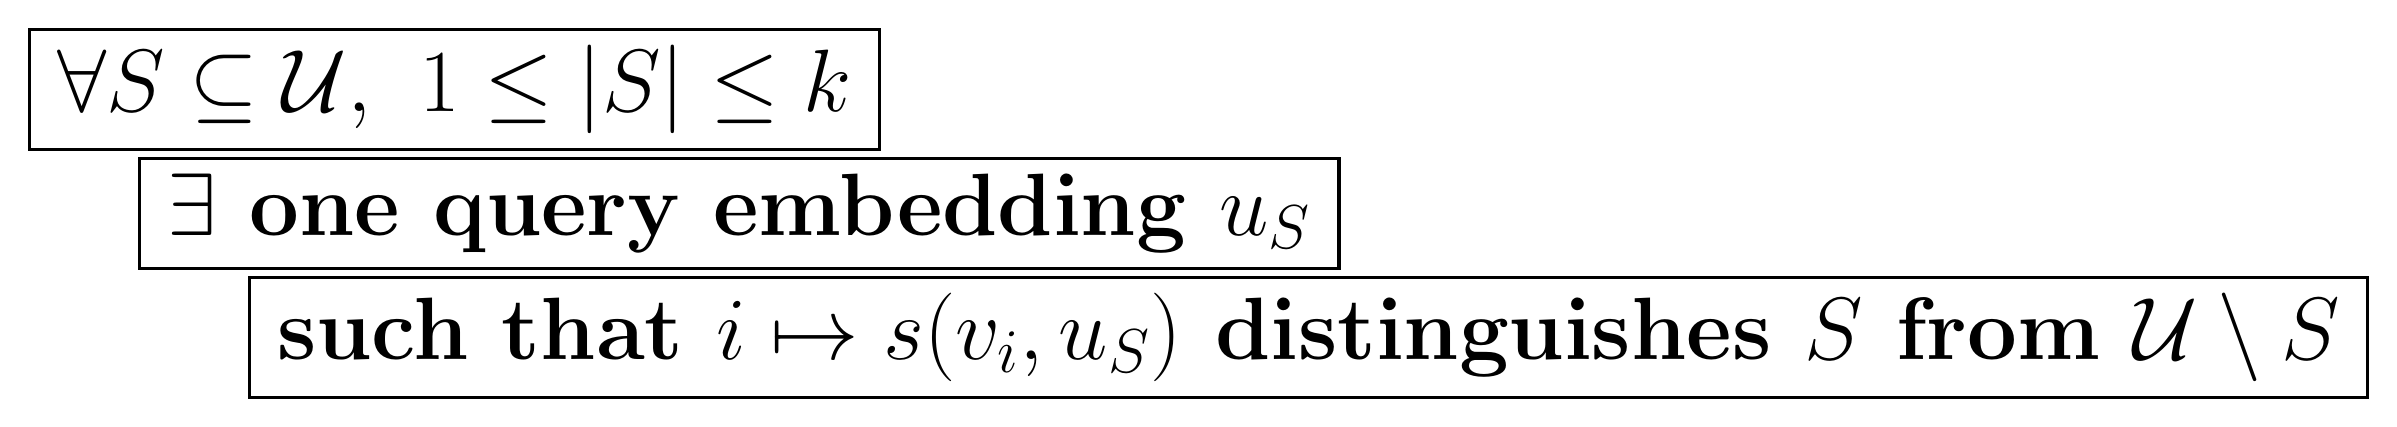
\begin{tikzpicture}[x=1in,y=1in]
        \node[draw=black,fill=white,line width=1.1pt,inner xsep=0.14in,inner ysep=0.08in,anchor=west]
          (forall) at (0,0) {{\MiniHeadFont $\forall S\subseteq\mathcal{U},\ 1\le |S|\le k$}};
        \node[draw=black,fill=white,line width=1.1pt,inner xsep=0.14in,inner ysep=0.08in,anchor=west]
          (exists) at (0.55,-0.62) {{\MiniHeadFont $\exists$ one query embedding $u_S$}};
        \node[draw=black,fill=white,line width=1.1pt,inner xsep=0.14in,inner ysep=0.08in,anchor=west]
          (such) at (1.1,-1.24) {{\MiniHeadFont such that $i\mapsto s(v_i,u_S)$
          distinguishes $S$ from $\mathcal{U}\setminus S$}};
        % \draw[->,line width=2pt] (forall.south west) -- (exists.west);
        % \draw[->,line width=2pt] (exists.south west) -- (such.west);
      \end{tikzpicture}
      \begin{itemize}[label=\textbullet,leftmargin=0.48in,labelsep=0.12in,itemsep=0.02in,topsep=0.02in,parsep=0pt]
        \item {\bfseries Minimal Embeddable Dimension (MED):}
        the smallest $d$ for which one shared configuration in
        $\mathbb{R}^d$ distinguishes every target set $|S|\le k$.
      \end{itemize}
      \end{center}
    \end{posterbox}

    \vspace{0.25in}
    \begin{posterbox}[defblock]
      {\SubheadFont Exact MED}\par\vspace{0.04in}
      {\centering\EquationFont
        $\displaystyle
        \min_{i\in S}s(v_i,u_S)>
        \max_{j\notin S}s(v_j,u_S)$\par}
      \vspace{0.04in}
      Strict ordering is enough. No prescribed margin or
      normalization is required.
    \end{posterbox}

    \vspace{0.25in}
    \begin{posterbox}[defblock]
      {\SubheadFont $\epsilon$-Robust MED}\par\vspace{0.04in}
      {\centering\EquationFont
        $\displaystyle
        \min_{i\in S}s(v_i,u_S)\ge
        \max_{j\notin S}s(v_j,u_S)+\epsilon$\par}
      \vspace{0.04in}
      Objects and queries are normalized, e.g. in unit ball. \\A uniform positive
      score gap must work for every target set.
    \end{posterbox}

    \vspace{0.25in}
    \begin{posterbox}[witnessblock]
      \begin{minipage}[t]{0.47\linewidth}
        {\MiniHeadFont\color{blue} Target set $S$}\par\vspace{0.1in}
        \begin{center}
        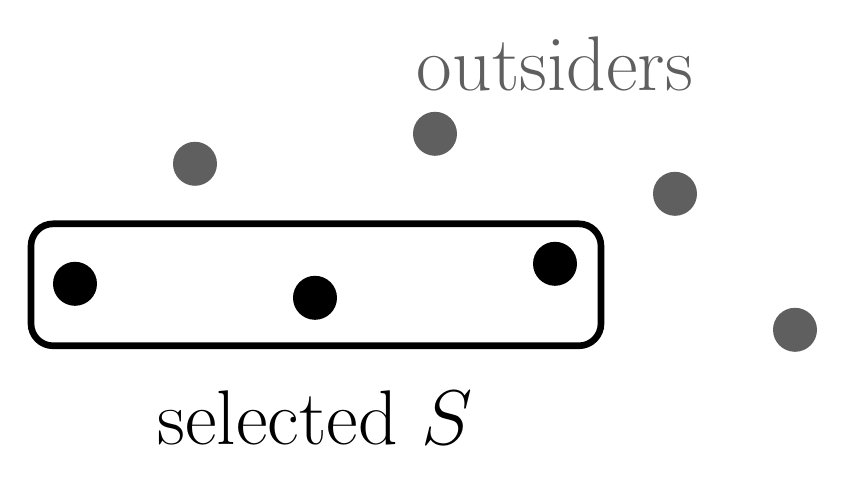
\begin{tikzpicture}[x=1in,y=1in]
          \foreach \x/\y/\c in {0.15/0.45/teal,0.75/1.05/muted,1.35/0.38/teal,1.95/1.2/muted,2.55/0.55/teal,3.15/0.9/muted,3.75/0.22/muted}
            \fill[\c] (\x,\y) circle (0.11);
          \draw[teal,line width=2.4pt,rounded corners=8pt] (-0.07,0.14) rectangle (2.78,0.75);
          \node[teal] at (1.35,-0.22) {\SmallFont selected $S$};
          \node[muted] at (2.55,1.55) {\SmallFont outsiders};
        \end{tikzpicture}
        \end{center}
        {\SmallFont Fixed object embeddings; the witness query $u_S$
        changes with $S$.}
      \end{minipage}\hfill
      \begin{minipage}[t]{0.49\linewidth}
        {\MiniHeadFont\color{amber} Score axis}\par\vspace{0.05in}
        \begin{center}
        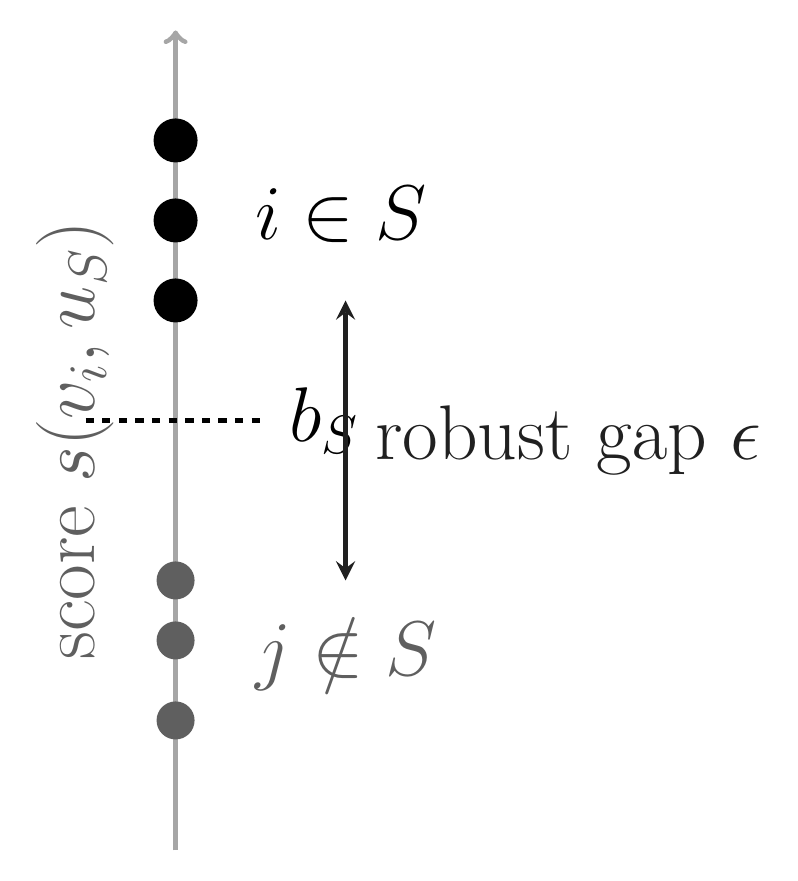
\begin{tikzpicture}[x=1in,y=1in]
          \draw[->,line width=2pt,gray!70] (1.6,0) -- (1.6,4.1);
          \node[rotate=90,muted] at (1.1,2.05) {\SmallFont score $s(v_i,u_S)$};
          \foreach \y in {0.65,1.05,1.35}
            \fill[muted] (1.6,\y) circle (0.095);
          \foreach \y in {2.75,3.15,3.55}
            \fill[teal] (1.6,\y) circle (0.11);
          \draw[teal,dashed,line width=2pt] (1.15,2.15) -- (2.05,2.15);
          \node[teal,anchor=west] at (2.12,2.15) {\SmallFont $b_S$};
          \draw[<->,>=stealth,line width=2pt,amber] (2.45,1.35) -- (2.45,2.75);
          \node[amber,anchor=west] at (2.55,2.05) {\SmallFont robust gap $\epsilon$};
          \node[teal,anchor=west] at (1.95,3.18) {\SmallFont $i\in S$};
          \node[muted,anchor=west] at (1.95,0.98) {\SmallFont $j\notin S$};
        \end{tikzpicture}
        \end{center}
      \end{minipage}
      \vspace{0.05in}
    \end{posterbox}

    \vspace{0.25in}
    \begin{posterbox}[defblock]
      {\SubheadFont VC lower bound}\par
      If all subsets of size at most $k$ can be realized, then the
      thresholded score class shatters any chosen $k$ objects. Thus
      \[
        k\le \mathrm{VCD}(\mathcal{C}_{s,d}).
      \]
      For inner-product and Euclidean threshold families,
      $\mathrm{VCD}=d+1$, so exact MED and every robust MED satisfy
      $d\ge k-1$.
    \end{posterbox}

    \begin{posterbox}[takeawayblock, height=1.45in, valign=center]
      \centering{\SubheadFont Lower bounds are $\Omega(k)$; the question is whether $m$ must enter.}
    \end{posterbox}
  \end{posterbox}
\end{minipage}\hfill
\begin{minipage}[t]{0.315\linewidth}
  \vspace{0pt}
  \begin{posterbox}
    \sectionhead{amber}{2. Theory}
    {\MiniHeadFont\color{amber} Exact capacity is $m$-independent; robust
    capacity pays for margin.}\par\vspace{0.12in}

    \begin{posterbox}[witnessblock]
      {\SubheadFont Cyclic-polytopal witness for Exact MED upper bound}\par
      Put all $m$ objects on the moment curve in $\mathbb{R}^{2k}$:
      \[
        v_i=(t_i,t_i^2,\ldots,t_i^{2k}),  \qquad 0 < t_1 < t_2 < \cdots < t_m < 1.
      \]
      For target $S$, consider the square polynomial $-P_S^2(t)$, where
      \[
        P_S(t) = \prod_{i\in S}(t-t_i).
      \]
      Note that $P_S^2$ has degree at most $2k$. Select $u_S$ from the
      nonconstant coefficients of $-P_S^2(t)$, giving a constant shift
      $c_S$:
      \[
        s(v_i,u_S)=\langle v_i,u_S\rangle=c_S-P_S^2(t_i)
        \begin{cases}
          =c_S, & i\in S,\\
          <c_S, & i\notin S.
        \end{cases}
      \]
    \end{posterbox}
    \vspace{0.22in}

    \begin{posterbox}[colback=teallight, colframe=teal]
      {\SubheadFont Exact MED theorem}\par\vspace{0.08in}
      {\TableFont
      \renewcommand{\arraystretch}{1.2}
      \begin{center}
        \begin{tabular}{>{\bfseries}lcc}
          \toprule
          Score & Lower & Upper \\
          \midrule
          Inner product & $k-1$ & $2k$ \\
          Euclidean & $k-1$ & $2k$ \\
          Cosine & $k-1$ & $2k+1$ \\
          \bottomrule
        \end{tabular}
      \end{center}
      }
      \par\vspace{0.08in}
      Main message: $\mathrm{MED}(m,k)=\Theta(k)$, independent
      of $m$ up to constants.
    \end{posterbox}

    \vspace{0.22in}
    \begin{posterbox}[colback=amberlight, colframe=amber]
      {\SubheadFont Feasible robust margin}\par\vspace{0.04in}
      \[
        \epsilon_\star(m,k)=
        \frac{m}{\sqrt{k(m-1)(m-k)}}
        \sim \frac{1}{\sqrt{k}}.
      \]
      If $\epsilon>\epsilon_\star(m,k)$, RMED is infinity.
      The ceiling is tight in $\mathbb{R}^{m-1}$ by a regular simplex.
    \end{posterbox}

    \vspace{0.22in}
    \begin{posterbox}[witnessblock]
      {\SubheadFont Gaussian centroid witness for robust MED upper bound}\par
      Sample random unit object vectors and query by normalized selected
      centroid:
      \[
        u_S=\frac{\sum_{i\in S}v_i}
        {\left\|\sum_{i\in S}v_i\right\|_2}.
      \]
      Selected objects get a self-correlation term; outsiders contribute
      coherence noise. With positive probability,
      \[
        d=Ck^2\log m
      \]
      robustly retrieves every at-most-$k$ subset with margin
      $\Omega(1/\sqrt{k})$.
    \end{posterbox}

    \vspace{0.16in}
    \begin{posterbox}[colback=amberlight, colframe=amber]
      {\SubheadFont RMED dimension ladder}\par\vspace{0.02in}
      { At $\epsilon_k=c/\sqrt{k}$, packing and Gaussian witnesses give}\vspace{-0.08in}
      {
      \[
      \begin{aligned}
        \max\!\left\{k-1,\frac{\log\binom{m}{k}}
        {\log(1+2/\epsilon)}\right\}
        &\le \mathrm{RMED}(m,k,\epsilon_k)
        &\le \mathrm{RMED\text{-}C}(m,k,\epsilon_k)\le Ck^2\log m .
      \end{aligned}
      \]
      }\vspace{-0.12in}
      { Packing supplies another lower bound for about $\log m$-dependent term.}
    \end{posterbox}

    \begin{posterbox}[takeawayblock, height=1.25in, valign=center]
      \centering{\SubheadFont $2k$ is enough for exact MED; $O(k^2\log m)$ is enough for robust MED.}
    \end{posterbox}
  \end{posterbox}
\end{minipage}\hfill
\begin{minipage}[t]{0.315\linewidth}
  \vspace{0pt}
  \begin{posterbox}
    \sectionhead{red}{3. Empirical}
    {\MiniHeadFont\color{red} Current ``hard'' datasets are easy to crack
    by explicit low-dimensional witnesses.}\par\vspace{0.12in}

    \begin{posterbox}[resultblock]
      {\color{blue}\SubheadFont Synthetic top-2: explicit $d=4$}\par\vspace{0.08in}
      \begin{center}
        \tightinclude[width=0.95\linewidth,height=6.45in,keepaspectratio]{../../paper/figures/top2_dimension_fit.pdf}
      \end{center}
      {\SmallFont At $m=640$, the cyclic construction checks
      $205120/205120$ singleton/pair queries.}
    \end{posterbox}

    \vspace{0.25in}
    \begin{posterbox}[resultblock]
      {\color{red}\SubheadFont LIMIT: random vectors outperform embedding
      models}\par\vspace{0.1in}
      \begin{center}
        \tightinclude[width=0.95\linewidth,height=5.5in,keepaspectratio]{../../paper/figures/limit_retrieval_limit.pdf}
      \end{center}
      \vspace{0.04in}
      \begin{center}
        \tightinclude[width=0.95\linewidth,height=5.5in,keepaspectratio]{../../paper/figures/limit_retrieval_limit_small.pdf}
      \end{center}
      \vspace{0.04in}
      \begin{center}
        {\TableFont
        \renewcommand{\arraystretch}{1.12}
        \begin{tabular}{>{\bfseries}lccc}
          \toprule
          Dataset & baseline & first vanilla $d$ & vanilla R@2 @4096 \\
          \midrule
          LIMIT & 0.030 & 512 & 0.7060 \\
          LIMIT-small & 0.543 & 512 & 0.9545 \\
          \bottomrule
        \end{tabular}}
      \end{center}
      \vspace{0.3in}
      {\SmallFont Vanilla token sums use no labels and no handcrafted phrases,
      yet exceed the strongest comparable single-vector Promptriever line.
      Handmade reaches R@2 $0.9980/1.0000$ at $d=4096$.}
    \end{posterbox}

    \begin{posterbox}[takeawayblock, height=1.65in, valign=center]
      {\SubheadFont Failures of embedding models DO NOT stress geometric capacity.}
    \end{posterbox}
  \end{posterbox}
\end{minipage}

\end{document}
